\documentclass[a1,landscape]{a0poster}
% \usepackage[margin={5cm,1cm,5cm,5cm}]{geometry}
\usepackage[left=5cm, right=5cm, top=7cm, bottom=2cm]{geometry}
\setlength\textwidth{78cm}
\usepackage[compact]{titlesec}

\usepackage{multicol} % This is so we can have multiple columns of text side-by-side
\columnsep=70pt % This is the amount of white space between the columns in the poster
\columnseprule=3pt % This is the thickness of the black line between the columns in the poster

\usepackage[svgnames]{xcolor} 

\usepackage{times} 

\usepackage{graphicx} % Required for including images
\graphicspath{{figures/}} % Location of the graphics files
\usepackage[font=small,labelfont=bf]{caption} % Required for specifying captions to tables and figures
\usepackage{amsfonts, amsmath, amsthm, amssymb} % For math fonts, symbols and environments
\usepackage{wrapfig} % Allows wrapping text around tables and figures

\begin{document}

\begin{minipage}[c]{0.9\linewidth}
\centering
\Huge \color{NavyBlue} \textbf{Question Answering with 2-Stage Candidate Selection} \color{Black}\\ % Title
\LARGE \textbf{Adam Davies \& Carlos Jimenez}\\ % Author(s)
\end{minipage}

\vspace{1cm} % A bit of extra whitespace between the header and poster content

%----------------------------------------------------------------------------------------

\begin{multicols}{3} % This is how many columns your poster will be broken into, a poster with many figures may benefit from less columns whereas a text-heavy poster benefits from more
\Large
%----------------------------------------------------------------------------------------
%	ABSTRACT
%----------------------------------------------------------------------------------------

\color{Navy} % Navy color for the abstract
\section*{\LARGE Introduction}
Question answering systems have been an historically important application for computer science in general, and one in which natural language processing plays a central role. Building successful systems typically requires combining multiple processes, including information retrieval techniques, classification, knowledge bases, dependency analysis, and other linguistic representations, with opportunities for boundless sophistication. 

%----------------------------------------------------------------------------------------
%	INTRODUCTION
%----------------------------------------------------------------------------------------

\color{SaddleBrown} % SaddleBrown color for the introduction

\section*{\LARGE Summary}
\textbf{Our objective} was to design a \textbf{single-document based question answering system}.\\
Our system follows a 2-stage approach. First, sentence selection, followed by answer identification, inspired by the approach outlined by Wang, Liu, Xiao et al.[1]. We used classification, lexical analysis, and a rule-based approach in the first stage, and argument, and semantic analysis in the second stage. Though our system could achieve fairly high recall, it was often at the expense of its precision. Improving the precision of our system proved to be a challenge, especially when trying to do so involved abandoning useful heuristics. 

\color{DarkSlateGray} % DarkSlateGray color for the rest of the content

\section*{\LARGE Tools Used}
\textbf{Natural Language Tool-Kit (NLTK)} - Formed the backbone of our text processing, and was integral to lexical analysis. \\
\textbf{Stanford CoreNLP} - Our primary parser for constituency parsing, and used for some Named Entity Recognition.\\
\textbf{Wordnet} - Interfaced through NLTK; wordnet was used to analyze similarity of sentences and arguments. \\
\textbf{SpaCy} - 

%----------------------------------------------------------------------------------------
%	MATERIALS AND METHODS
%----------------------------------------------------------------------------------------

\section*{\LARGE First Stage - Sentence Selection}
Our first stage required question classification into questions of type who, what, which, when, where, why, and how. This enabled us to treat each case differently, and additionally deal with particular sub-cases. \\
Sub-cases of question types were often dealt with in a rule-based manner, especially when using NER. For example, if we know we are dealing with a how-much question, we can often identify candidate sentences by those containing MONEY patterns, or finally just CARDINAl entities. After narrowing down the pool of candidates, we filter our candidate pool through more general sentence selection subprocesses. \\
\textbf{The "general" case} - Our system has two generalized processes when either dealing with questions which we cannot assign a sub-case, or after narrowing the candidate pool and we need to rank candidates.\\ For example, one process involved lemmatizing and extracting significant words from a sentence, while preserving their POS tags, and comparing them with those words in the question processed the same way. Sentences are then ranked by their overlap, and passed on to the second stage (answer identification).
\begin{center}\vspace{1cm}
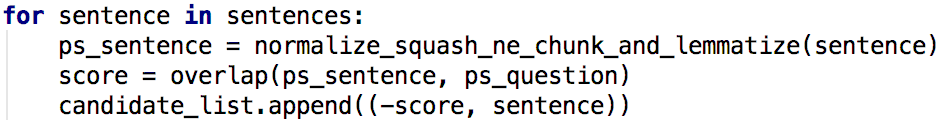
\includegraphics[width=0.85\linewidth]{snippet1.png}
\captionof{figure}{\color{Black} General Sentence Selection 1}
\end{center}\vspace{1cm}

%------------------------------------------------

\section*{\LARGE Second Stage - Answer Candidate Selection}

Nulla vel nisl sed mauris auctor mollis non sed. 

Curabitur mi sem, pulvinar quis aliquam rutrum. (1) edf (2)
, $\Omega=[-1,1]^3$, maecenas leo est, ornare at. $z=-1$ edf $z=1$ sed interdum felis dapibus sem. $x$ set $y$ ytruem. 


%----------------------------------------------------------------------------------------
%	RESULTS 
%----------------------------------------------------------------------------------------
\section*{\LARGE Results}

Donec faucibus purus at tortor egestas eu fermentum dolor facilisis. Maecenas tempor dui eu neque fringilla rutrum. Mauris \emph{lobortis} nisl accumsan. Aenean vitae risus ante. Pellentesque condimentum dui. Etiam sagittis purus non tellus tempor volutpat. Donec et dui non massa tristique adipiscing.


Nulla ut porttitor enim. Suspendisse venenatis dui eget eros gravida tempor. Mauris feugiat elit et augue placerat ultrices. Morbi accumsan enim nec tortor consectetur non commodo. Pellentesque condimentum dui. Etiam sagittis purus non tellus tempor volutpat. Donec et dui non massa tristique adipiscing. 

In hac habitasse platea dictumst. Etiam placerat, risus ac.

Adipiscing lectus in magna blandit:

Vivamus sed nibh ac metus tristique tristique a vitae ante. Sed lobortis mi ut arcu fringilla et adipiscing ligula rutrum. Aenean turpis velit, placerat eget tincidunt nec, ornare in nisl. In placerat.

%----------------------------------------------------------------------------------------
%	CONCLUSIONS
%----------------------------------------------------------------------------------------

\color{SaddleBrown} % SaddleBrown color for the conclusions to make them stand out

\section*{\LARGE Conclusions}
\textbf{What Worked Well}
\begin{itemize}
    \item Heuristics and a rule-based approach were hard to abandon.
    \item 
\end{itemize}
\vspace{0.7em}
\textbf{What Did Not}
\begin{itemize}
    \item 
\end{itemize}

\color{DarkSlateGray} % Set the color back to DarkSlateGray for the rest of the content

 %----------------------------------------------------------------------------------------
%	REFERENCES
%----------------------------------------------------------------------------------------

\nocite{*} % Print all references regardless of whether they were cited in the poster or not
\bibliographystyle{plain} % Plain referencing style
\bibliography{sample} % Use the example bibliography file sample.bib

\end{multicols}
\end{document}